\section{Casi d'uso}
Di seguito vengono riportati i casi d'uso raggruppati in base all'attore. Gli attori in gioco sono i seguenti:
\begin{itemize}
	\item volontario;
	\item caposquadra;
	\item coordinatore.
\end{itemize}

\subsection{Casi d'uso: Volontario}
\begin{itemize}
	\item \textbf{UC1 - Login}:
	come volontario, voglio poter accedere al mio profilo personale.
	
	\item \textbf{UC2 - Logout}:
	come volontario, voglio poter disconnettere il mio profilo personale dall'applicazione.
	
	\item \textbf{UC3 - Visualizzazione informazioni account}:
	come volontario, voglio poter accedere alle informazioni relative al mio account.
	
	\item \textbf{UC4 - Visualizzazione informazioni squadra}:
	come volontario, voglio poter accedere alle informazioni relative alla mia squadra.
	
	\item \textbf{UC5 - Gestione reperibilità}:
	come volontario, voglio poter indicare e modificare le mie ore di reperibilità.
	
	\item \textbf{UC6 - Segnalazione operatività}:
	come volontario, voglio poter segnalare quando sono operativo e mi trovo sul luogo dell'intervento.
	
	\item \textbf{UC7 - Visualizzazione intervento di emergenza}:
	come volontario, voglio poter visualizzare le informazioni relative ad un intervento di emergenza a cui sono stato assegnato.
	
	\item \textbf{UC8 - Visualizzazione intervento programmato}:
	come volontario, voglio poter visualizzare le informazioni relative ad un intervento programmato a cui sono stato assegnato.
	
	\item \textbf{UC9 - Inserimento informazioni intervento}:
	come volontario, voglio poter arricchire la documentazione relativa all'intervento, programmato oppure di emergenza, a cui sono stato assegnato aggiungendo foto e osservazioni.
	
	\item \textbf{UC10 - Visualizzazione posizione real-time}:
	come volontario, voglio poter visualizzare su una mappa la posizione in tempo reale dei colleghi operativi appartenenti alla mia squadra durante un intervento.
	
	\item \textbf{UC18 - Visualizzazione informazioni zona}:
	come volontario, voglio poter consultare le informazioni riguardanti il meteo, i terremoti, la qualità dell'aria, le stazioni personalizzate e gli allarmi relativi alla zona assegnata alla mia squadra.
\end{itemize}




\subsection{Casi d'uso: Caposquadra}
Il caposquadra include tutti i casi d'uso del volontario più i seguenti:
\begin{itemize}
	\item \textbf{UC11 - Gestione intervento di emergenza}:
	come caposquadra, voglio poter creare, modificare o eliminare un intervento di emergenza.
	
	\item \textbf{UC12 - Gestione intervento programmato}:
	come caposquadra, voglio poter creare, modificare o eliminare un intervento programmato.
	
	\item \textbf{UC13 - Gestione report intervento di emergenza}:
	come caposquadra, voglio poter visualizzare e modificare i report riguardanti gli interventi di emergenza creati da me.
	
	\item \textbf{UC14 - Gestione report intervento programmato}:
	come caposquadra, voglio poter visualizzare e modificare i report riguardanti gli interventi programmati creati da me.
		
	\item \textbf{UC19 - Notifiche allarmi zona}:
	come caposquadra, voglio poter decidere su quali  allarmi relativi alla mia zona essere notificato.
	
	\item \textbf{UC20 - Gestione informazioni relative alla zona}:
	come caposquadra, voglio poter inserire, modificare ed eliminare i dati delle stazioni APRS da cui ricevere i dati.
\end{itemize}

\subsection{Casi d'uso: Coordinatore}
\begin{itemize}
	\item \textbf{UC1 - Login}:
	come coordinatore, voglio poter accedere al mio profilo personale.
	
	\item \textbf{UC2 - Logout}:
	come coordinatore, voglio poter disconnettere il mio profilo personale dall'applicazione.
	
	\item \textbf{UC3 - Visualizzazione informazioni account}:
	come coordinatore, voglio poter accedere alle informazioni relative al mio account.
	
	\item \textbf{UC4 - Visualizzazione informazioni squadra}:
	come coordinatore, voglio poter accedere alle informazioni relative alle squadre da me create.
	
	\item \textbf{UC15 - Inserimento utente}:
	come coordinatore, voglio poter inserire un nuovo utente.
	
	\item \textbf{UC16 - Cancellazione utente}:
	come coordinatore, voglio poter cancellare un utente.
	
	\item \textbf{UC17 - Gestione squadre}:
	come coordinatore, voglio poter creare, modificare, eliminare le squadre e assegnare a ognuna di esse un caposquadra.
\end{itemize}

\clearpage
\subsection{Diagramma dei casi d'uso}
In figura \ref{fig:UseCaseDiagram} è stato riportato il diagramma dei casi d'uso. In questo diagramma sono stati inseriti i casi d'uso descritti in precedenza mettendoli in correlazione con il corrispettivo attore. È importante notare che la figura del \textit{caposquadra} è una specializzazione del \textit{volontario} e di conseguenza eredita tutti i suoi casi d'uso, oltre ad implementarne altri personalizzati. 
\begin{landscape}
	\begin{figure}[b]
		\centering
		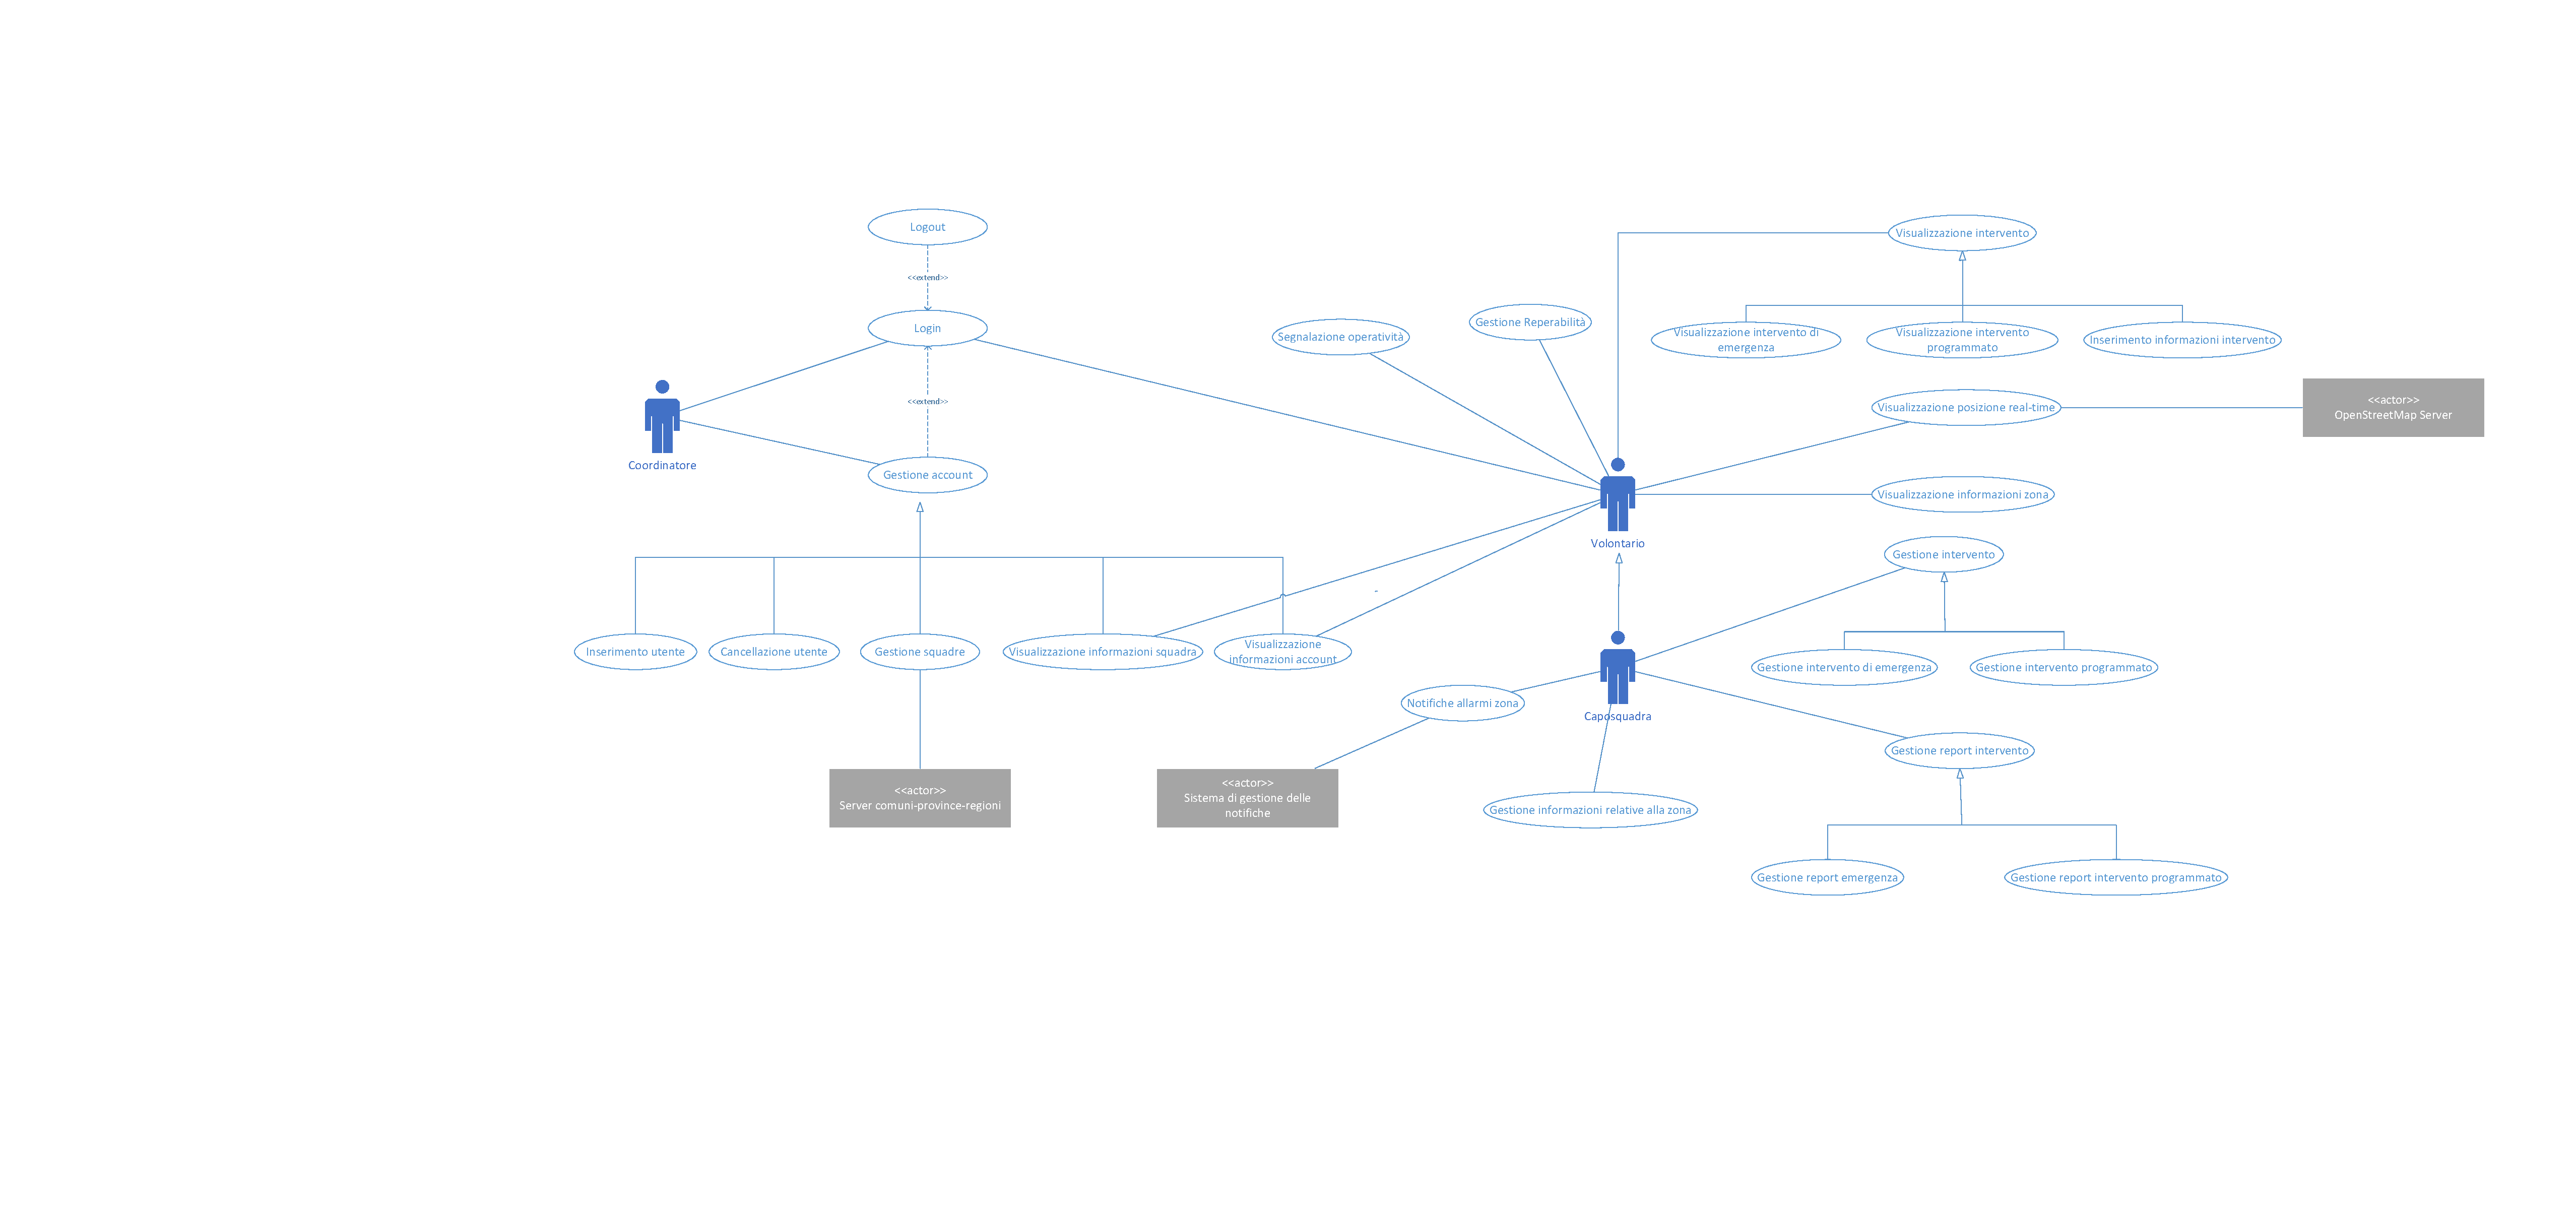
\includegraphics[width=1\linewidth]{./Iterazione 0/OtherFiles/Use cases diagram}
		\caption{Diagramma dei casi d'uso.}
		\label{fig:UseCaseDiagram}
	\end{figure}
\end{landscape}

